\documentclass[aspectratio=169]{beamer}

% --- PACOTES BÁSICOS ---
\usepackage[utf8]{inputenc}
\usepackage[portuguese]{babel}
\usepackage{amsmath, amssymb}
\usepackage{booktabs}
\usepackage{graphicx}
\usepackage{helvet}
\usepackage{tikz}
\usepackage{xcolor}
\usepackage{colortbl}
\usepackage{pgfplots}
\pgfplotsset{compat=1.18}
\usepackage{microtype}   % Melhora justificação e reduz overfull hbox

% --- TEMA BEAMER ---
\usetheme{Madrid}
\usecolortheme{whale}

% Paleta de cores UFRN
\definecolor{ufrnblue}{RGB}{10, 58, 96}
\definecolor{accentblue}{RGB}{30, 144, 255}
\definecolor{positivegreen}{RGB}{0, 153, 76}
\definecolor{warnyellow}{RGB}{204, 153, 0}
\definecolor{negred}{RGB}{180, 30, 30}
\definecolor{lightgray}{RGB}{240, 240, 240}

\setbeamercolor{palette primary}{bg=ufrnblue, fg=white}
\setbeamercolor{palette secondary}{bg=accentblue, fg=white}
\setbeamercolor{palette tertiary}{bg=ufrnblue, fg=white}
\setbeamercolor{titlelike}{parent=palette primary}
\setbeamercolor{structure}{fg=ufrnblue}
\setbeamercolor{block title}{bg=ufrnblue, fg=white}
\setbeamercolor{block body}{bg=ufrnblue!8}
\setbeamercolor{alerted text}{fg=negred}

% Remove ícones de navegação; mostra número de frame limpo
\setbeamertemplate{navigation symbols}{}
\setbeamertemplate{footline}[frame number]

% --- METADADOS ---
\title[Clustering \& LLM]{Agrupamento de Notícias com Análise por LLM}
\subtitle{Representações Frequenciais e Semânticas · 4 Algoritmos · Explicação Automática}
\author[Cauã Vitor]{Cauã Vitor\\{\small Orientador: Prof.\ José Alfredo F.\ Costa}}
\institute[UFRN]{Universidade Federal do Rio Grande do Norte\\Departamento de Engenharia de Computação e Automação (DCA)}
\date[Jun/2026]{Junho de 2026}

\begin{document}

% =============================================
% Slide 1: Capa
% =============================================
\begin{frame}
  \titlepage
\end{frame}

% =============================================
% Slide 2: Roteiro
% =============================================
\begin{frame}{Roteiro da Apresentação}
  \tableofcontents[hideallsubsections]
\end{frame}

% =============================================
\section{Motivação e Objetivo}
% =============================================
\begin{frame}{Motivação e Objetivo}
  \begin{columns}[T]
    \begin{column}{0.56\textwidth}
      \begin{itemize}
        \item \textbf{Problema:} Agrupar notícias em categorias temáticas
              \emph{sem supervisão humana} — tarefa clássica e desafiadora em PLN.
        \item \textbf{Dataset:} 315 notícias em português, \textbf{6 classes}:
        \begin{itemize}\small
          \item Economia, Esportes, Política
          \item Polícia e Direitos, Turismo
          \item Variedades e Sociedade
        \end{itemize}
        \item \textbf{Questão de Pesquisa:} Qual representação vetorial e qual
              algoritmo produz grupos mais coerentes com a semântica humana?
      \end{itemize}
    \end{column}
    \begin{column}{0.42\textwidth}
      \begin{block}{Pipeline do Experimento}
        \small
        \begin{enumerate}
          \item Vetorização: TF-IDF vs Embeddings
          \item Clustering: 4 algoritmos × 3 representações
          \item Projeção 2D: PCA, t-SNE, UMAP
          \item Seleção de landmarks (medoides/fronteiras)
          \item Explicação semântica via LLM
        \end{enumerate}
      \end{block}
    \end{column}
  \end{columns}
\end{frame}

% =============================================
\section{Representações Vetoriais}
% =============================================
\begin{frame}{Representações Vetoriais de Texto}
  \begin{columns}[T]
    \begin{column}{0.48\textwidth}
      \textbf{\color{ufrnblue}TF-IDF (Frequencial)}
      \begin{itemize}
        \item Clássico \textit{bag-of-words}: ignora contexto semântico
        \item Vocabulário: até \textbf{1.000 termos} após remoção de
              \textit{stopwords} em PT
        \item Vetores esparsos de alta dimensão
      \end{itemize}
      \[ \mathrm{TF\text{-}IDF}(t,d,D) = \mathrm{tf}(t,d)\cdot
         \log\!\left(\tfrac{|D|}{1+|\{d:t\in d\}|}\right) \]
    \end{column}
    \begin{column}{0.50\textwidth}
      \textbf{\color{ufrnblue}Embeddings Semânticos Densos}
      \begin{itemize}
        \item Redes neurais que capturam sinônimos, contexto e relações implícitas
        \item \textbf{Sentence Transformers:}\\
              \texttt{\small paraphrase-multilingual-MiniLM-L12-v2}\\
              384 dim — \alert{treinado em PT-BR}
        \item \textbf{Ollama (local):}\\
              \texttt{nomic-embed-text} — 768 dim
      \end{itemize}
    \end{column}
  \end{columns}
\end{frame}

% =============================================
\section{Algoritmos de Clustering}
% =============================================
\begin{frame}{Algoritmos de Agrupamento Testados}
  \begin{columns}[T]
    \begin{column}{0.48\textwidth}
      \begin{block}{K-Means}
        \small Particional. Minimiza inércia intra-cluster.
        Assume grupos convexos de tamanho similar ($K=6$).
      \end{block}
      \vspace{0.4em}
      \begin{block}{Agglomerative (Ward)}
        \small Hierárquico ascendente (\textit{bottom-up}).
        Mescla pares pelo critério de Ward: menor variância intra-grupo.
      \end{block}
    \end{column}
    \begin{column}{0.48\textwidth}
      \begin{block}{DBSCAN}
        \small Baseado em densidade. Classifica pontos isolados como
        ruído ($-1$). Sensível ao parâmetro $\varepsilon$ e à
        dimensionalidade.
      \end{block}
      \vspace{0.4em}
      \begin{block}{HDBSCAN}
        \small Extensão hierárquica do DBSCAN. Suporta densidades
        variáveis sem $\varepsilon$ fixo. Mais robusto a \textit{outliers}.
      \end{block}
    \end{column}
  \end{columns}
\end{frame}

% =============================================
\section{Métricas de Avaliação}
% =============================================
\begin{frame}{Métricas de Validação do Clustering}
  \begin{columns}[T]
    \begin{column}{0.50\textwidth}
      \textbf{\color{ufrnblue}Não Supervisionadas}
      \begin{itemize}
        \item \textbf{Coeficiente de Silhueta} $s(i)\in[-1,+1]$:
        \[ s(i) = \frac{b(i)-a(i)}{\max\bigl(a(i),b(i)\bigr)} \]
        $a(i)$: distância média intra-cluster; $b(i)$: distância média
        ao cluster vizinho mais próximo.
        \item \textbf{Davies-Bouldin} $\downarrow$: clusters mais
              compactos e separados.
      \end{itemize}
    \end{column}
    \begin{column}{0.48\textwidth}
      \textbf{\color{ufrnblue}Supervisionadas (vs.\ Ground Truth)}
      \begin{itemize}
        \item \textbf{ARI} (Adjusted Rand Index): concordância
              corrigida pelo acaso. Ideal $=1{,}0$.
        \item \textbf{NMI} (Normalized Mutual Info): alinhamento
              via teoria da informação. Varia em $[0,1]$.
        \item \textbf{Pureza}: fração das amostras na classe majoritária
              de cada cluster.
      \end{itemize}
    \end{column}
  \end{columns}
\end{frame}

% =============================================
\section{Resultados Experimentais}
% =============================================
\begin{frame}{Resultados Quantitativos — 12 Configurações}
  {\footnotesize
  \begin{table}[h]
    \centering
    \setlength{\tabcolsep}{5pt}
    \renewcommand{\arraystretch}{1.15}
    \begin{tabular}{llcccc}
      \toprule
      \textbf{Representação} & \textbf{Algoritmo} &
      \textbf{Silhueta} & \textbf{ARI\,↑} & \textbf{NMI\,↑} & \textbf{Pureza\,↑}\\
      \midrule
      \rowcolor{positivegreen!20}
      TF-IDF & \textbf{Agglomerative} & 0{,}025 & \textbf{0{,}852} & \textbf{0{,}852} & \textbf{0{,}933}\\
      TF-IDF & K-Means               & 0{,}024 & 0{,}705 & 0{,}778 & 0{,}857\\
      TF-IDF & DBSCAN                & 0{,}007 & 0{,}029 & 0{,}369 & 0{,}994\textsuperscript{*}\\
      TF-IDF & HDBSCAN               & 0{,}002 & 0{,}004 & 0{,}048 & 0{,}317\\
      \midrule
      SentTransf.\ (PT-BR) & K-Means        & 0{,}083 & 0{,}556 & 0{,}665 & 0{,}752\\
      SentTransf.\ (PT-BR) & Agglomerative  & 0{,}079 & 0{,}587 & 0{,}743 & 0{,}756\\
      \midrule
      Ollama (nomic) & K-Means       & 0{,}064 & 0{,}500 & 0{,}616 & 0{,}724\\
      Ollama (nomic) & Agglomerative & 0{,}056 & 0{,}455 & 0{,}564 & 0{,}695\\
      \bottomrule
    \end{tabular}
    \vspace{0.3em}\\
    {\tiny \textsuperscript{*}Pureza inflada: DBSCAN concentrou maioria das amostras
     em clusters ruidosos. Pipeline executado em Junho/2026 com 315 notícias.}
  \end{table}
  }
  \vspace{-0.5em}
  \begin{block}{\small Destaque}
    \small \textbf{TF-IDF + Agglomerative} alcançou o maior ARI (0{,}852) e Pureza
    (0{,}933), superando embeddings semânticos neste corpus.
  \end{block}
\end{frame}

% =============================================
% Slide: Visualização de ARI por configuração
% =============================================
\begin{frame}{Comparativo Visual de ARI por Configuração}
  \begin{columns}[T]
    \begin{column}{0.60\textwidth}
      \begin{tikzpicture}
        \begin{axis}[
          xbar,
          width=7.5cm, height=5.8cm,
          xlabel={\small ARI},
          xmin=0, xmax=1.0,
          symbolic y coords={
            {Ollama+Agg},
            {Ollama+KM},
            {TF-IDF+HDBSCAN},
            {TF-IDF+DBSCAN},
            {ST+KM},
            {ST+Agg},
            {TF-IDF+KM},
            {TF-IDF+Agg}
          },
          ytick=data,
          yticklabel style={font=\tiny},
          xticklabel style={font=\tiny},
          xlabel style={font=\small},
          nodes near coords,
          nodes near coords style={font=\tiny, anchor=west},
          every node near coord/.append style={xshift=1pt},
          bar width=5pt,
          enlarge y limits=0.08,
          grid=major,
          grid style={dashed, gray!30},
        ]
          \addplot[fill=ufrnblue!70, draw=ufrnblue] coordinates {
            ({0.455},{Ollama+Agg})
            ({0.500},{Ollama+KM})
            ({0.004},{TF-IDF+HDBSCAN})
            ({0.029},{TF-IDF+DBSCAN})
            ({0.556},{ST+KM})
            ({0.587},{ST+Agg})
            ({0.705},{TF-IDF+KM})
            ({0.852},{TF-IDF+Agg})
          };
          % Destaque barra vencedora
          \addplot[fill=positivegreen!80, draw=positivegreen] coordinates {
            ({0.852},{TF-IDF+Agg})
          };
        \end{axis}
      \end{tikzpicture}
    \end{column}
    \begin{column}{0.38\textwidth}
      \begin{itemize}\small
        \item \textbf{\color{positivegreen}TF-IDF + Agglomerative} é o vencedor
              absoluto em ARI e NMI
        \item \textbf{DBSCAN e HDBSCAN} colapam em espaços de alta dimensão
              (maldição da dimensionalidade)
        \item Embeddings semânticos têm Silhueta maior ($\approx 0{,}08$)
              mas ARI menor — melhor separação geométrica, pior alinhamento
              com a taxonomia humana
      \end{itemize}
    \end{column}
  \end{columns}
\end{frame}

% =============================================
% Slide: Por que TF-IDF ganhou?
% =============================================
\begin{frame}{Por que o TF-IDF Superou os Embeddings?}
  \begin{columns}[T]
    \begin{column}{0.56\textwidth}
      \begin{itemize}
        \item \textbf{Corpus pequeno (315 amostras):} vocabulário jornalístico
              específico por categoria — ``gol'', ``voto'', ``inflação'' — é
              capturado diretamente pelo TF-IDF.
        \item \textbf{Linkage de Ward:} minimiza variância intra-grupo e é
              particularmente eficaz para vetores esparsos de alta dimensão.
        \item \textbf{Embeddings — limitações:}
        \begin{itemize}
          \item \texttt{all-MiniLM-L6-v2} (inglês) gerava embeddings subótimos
                para PT-BR.
          \item Modelo atual (\texttt{multilingual-MiniLM}) melhora ARI
                de $\approx 0{,}34$ para \textbf{0{,}587} no Agglomerative.
        \end{itemize}
      \end{itemize}
    \end{column}
    \begin{column}{0.42\textwidth}
      \begin{alertblock}{Paradoxo Silhueta vs.\ ARI}
        \small TF-IDF tem Silhueta $\approx 0{,}02$ (vetores esparsos
        geometricamente sobrepostos), mas ARI $= 0{,}852$.
        Ward detecta padrões corretos via distâncias de Ward
        mesmo sem separação euclidiana nítida.
      \end{alertblock}
      \vspace{0.4em}
      \begin{block}{\small DBSCAN/HDBSCAN}
        \small Alta dimensão $\Rightarrow$ distâncias euclidianas tornam-se
        indistinguíveis: regiões densas desaparecem.
      \end{block}
    \end{column}
  \end{columns}
\end{frame}

% =============================================
% Slide: Visualização 2D
% =============================================
\begin{frame}{Projeção 2D — Visualização dos Clusters}
  \begin{columns}[T]
    \begin{column}{0.60\textwidth}
      \begin{figure}
        \centering
        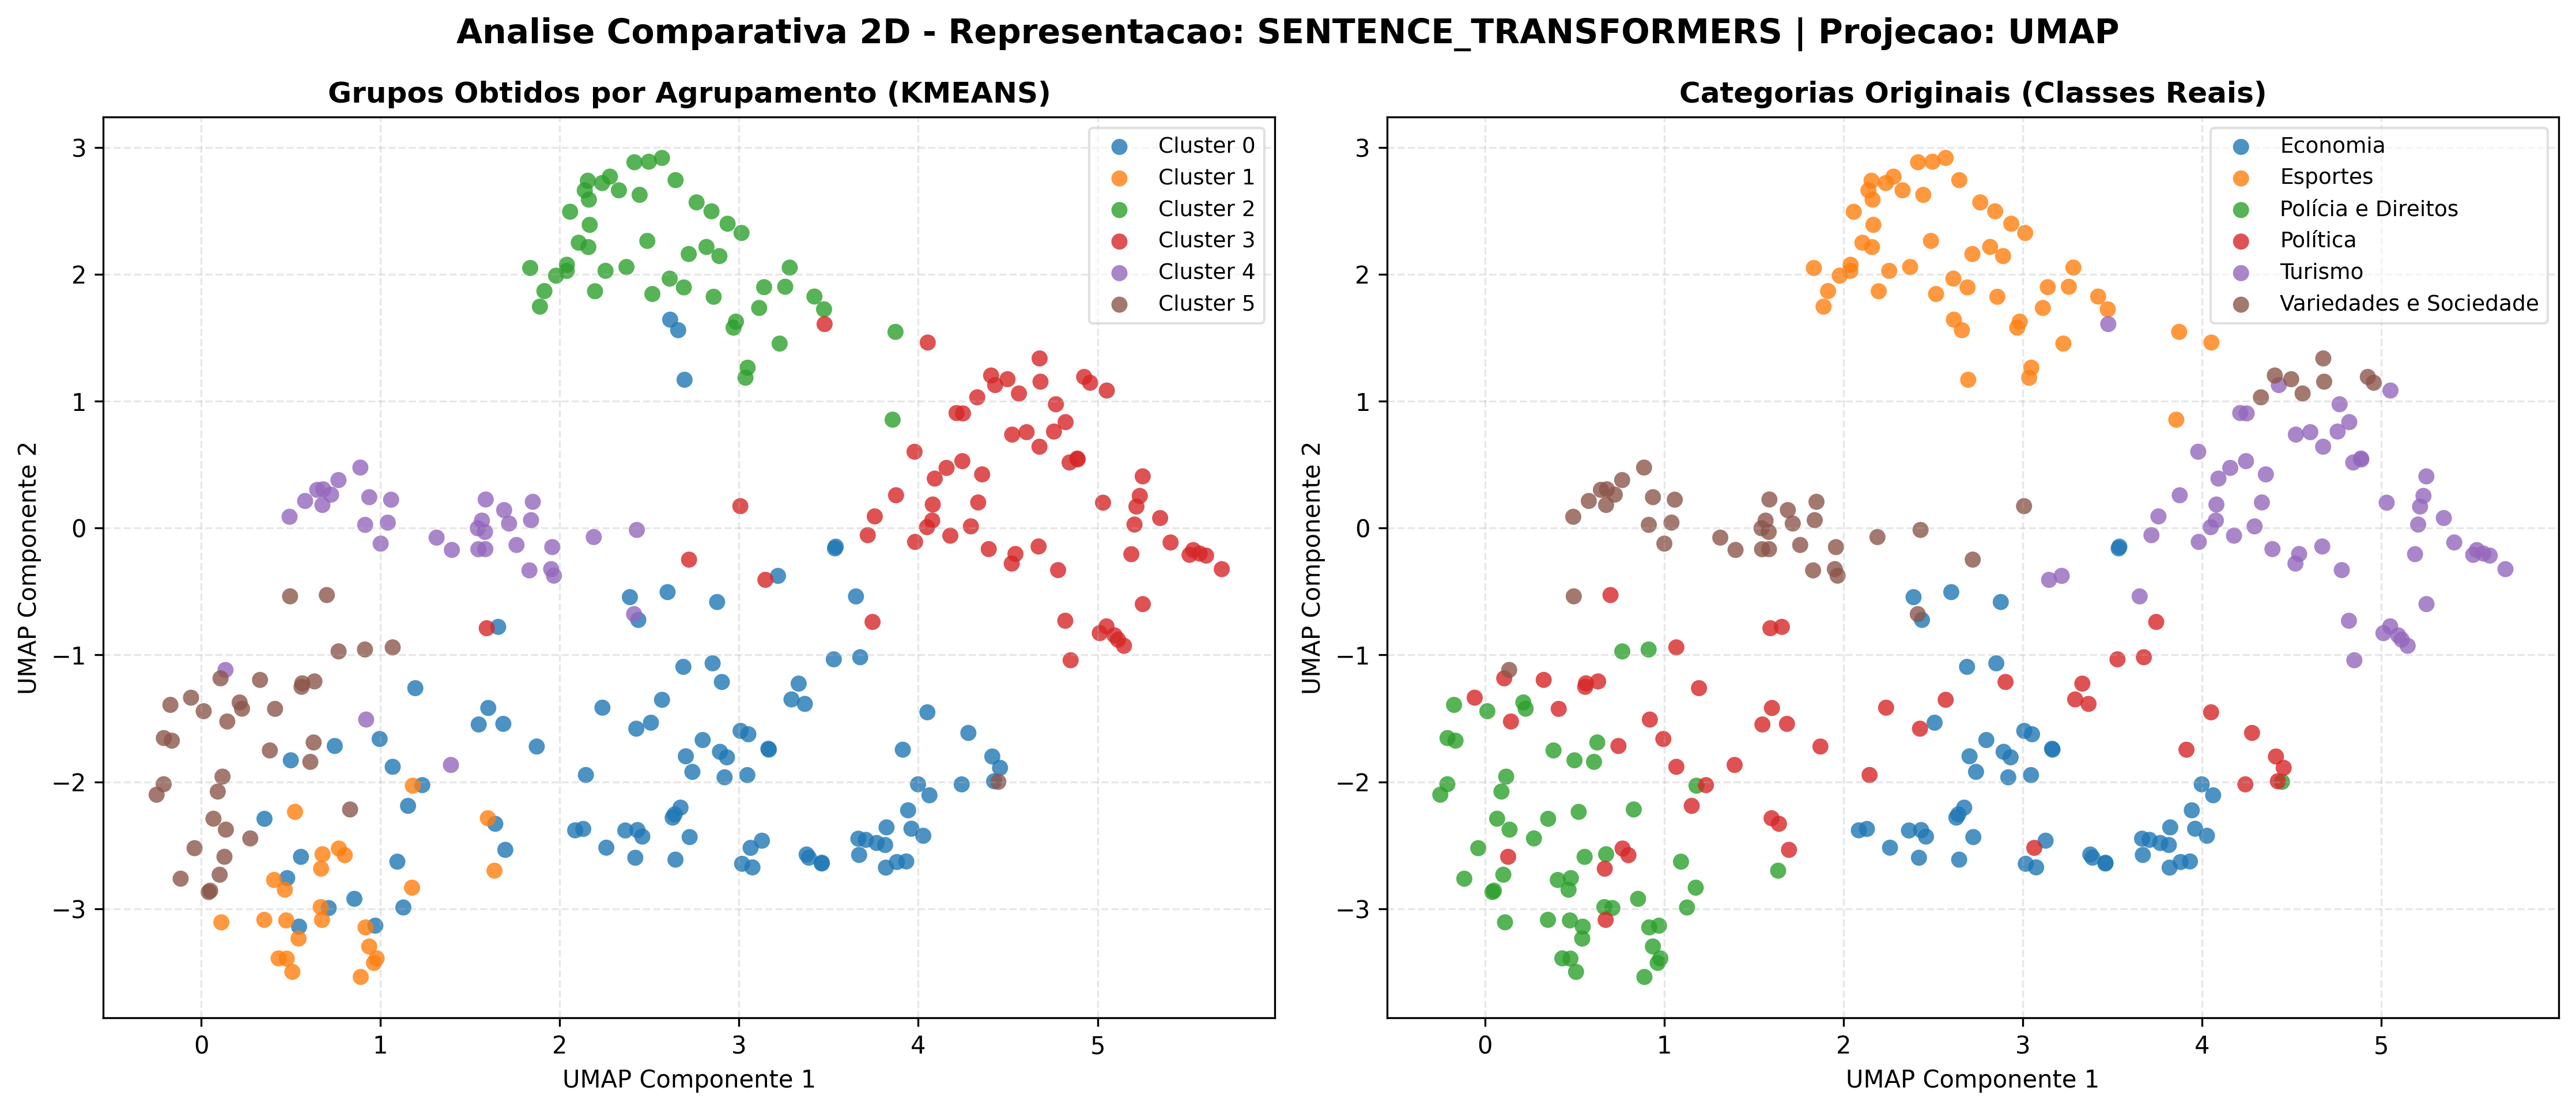
\includegraphics[width=\linewidth]{../backend/outputs/comparacao_agrupamento_umap.png}
        \caption{\footnotesize Projeção UMAP. Esquerda: clusters preditos.
                 Direita: classes reais (\textit{ground truth}).}
      \end{figure}
    \end{column}
    \begin{column}{0.38\textwidth}
      \begin{itemize}\small
        \item \textbf{PCA:} Linear. Preserva variância global; não captura
              estruturas não-lineares.
        \item \textbf{t-SNE:} Preserva vizinhança local. Excelente para
              inspeção visual — não preserva distâncias globais.
        \item \textbf{UMAP:} Equilíbrio local/global. Topologia mais natural
              do espaço semântico.
        \item Dashboard React permite transitar entre as 3 projeções com
              animação de \textit{morphing} suave.
      \end{itemize}
    \end{column}
  \end{columns}
\end{frame}

% =============================================
\section{Explicação Semântica via LLM}
% =============================================
\begin{frame}{Seleção de Landmarks e Explicação por LLM}
  \begin{columns}[T]
    \begin{column}{0.50\textwidth}
      \textbf{\color{ufrnblue}Seleção de Amostras-Chave}
      \begin{itemize}
        \item \textbf{Medoides (centrais):} menor distância euclidiana ao
              centroide — núcleo puro do tema.
        \item \textbf{Fronteiras (ambíguos):} menor coeficiente de silhueta
              individual ($s \approx 0$ ou negativo) — textos com interseção
              temática entre clusters.
      \end{itemize}
      \vspace{0.4em}
      \begin{exampleblock}{\small Saída JSON do LLM}
        \tiny\texttt{\{"rotulo": "Economia Verde",\\
        "resumo": "...", "coerencia": "Alta"\}}
      \end{exampleblock}
    \end{column}
    \begin{column}{0.48\textwidth}
      \textbf{\color{ufrnblue}Pipeline de Explicação}
      \begin{enumerate}\small
        \item Selecionar 3 medoides + 3 fronteiristas por cluster
        \item Montar prompt estruturado em PT com o texto das amostras
        \item Chamar \textbf{Ollama local} (Qwen 2.5 7B) \emph{e}
              \textbf{Gemma 4 31B} (nuvem) em paralelo
        \item Parsear JSON: \texttt{rotulo}, \texttt{resumo},
              \texttt{analise\_fronteira}, \texttt{coerencia}
        \item Retry exponencial contra erros 503; \textit{fail-fast} em cota 429
      \end{enumerate}
    \end{column}
  \end{columns}
\end{frame}

% =============================================
% Slide: Tabela de rótulos LLM
% =============================================
\begin{frame}{Rótulos Gerados pelos LLMs (TF-IDF + Agglomerative)}
  {\small
  \begin{table}
    \centering
    \setlength{\tabcolsep}{4pt}
    \renewcommand{\arraystretch}{1.2}
    \begin{tabular}{clll}
      \toprule
      \textbf{\#} & \textbf{Classe Real Dominante} &
      \textbf{Ollama (Qwen 2.5)} & \textbf{Gemma 4 31B}\\
      \midrule
      0 & Variedades e Sociedade & Cultura e Desenvolvimento   & Cultura e Capacitação\\
      1 & Esportes               & Esportes e Aventura          & Esportes e Ecoturismo\\
      2 & Política               & Política Social              & Política e Governança\\
      3 & Polícia e Direitos     & Direitos Humanos             & Políticas de Direitos\\
      4 & Turismo / Cultura      & Cultura e Economia Criativa  & Cultura e Econ.\ Criativa\\
      5 & Economia               & Economia Verde               & Economia e Sustentabilidade\\
      \bottomrule
    \end{tabular}
    \caption{\footnotesize Rótulos semânticos gerados via LLM para a melhor
             configuração (TF-IDF + Agglomerative, Pureza 0{,}933).}
  \end{table}
  }
  \vspace{-0.4em}
  \begin{block}{\small Observação}
    \small Ambos os modelos convergiram para rótulos semanticamente
    coerentes com as categorias humanas. Gemma 4 31B produziu rótulos
    ligeiramente mais descritivos; Qwen 2.5 7B foi mais conciso.
  \end{block}
\end{frame}

% =============================================
% Slide: LLM Local vs Nuvem
% =============================================
\begin{frame}{LLM Local (Ollama) vs.\ Nuvem (Gemini/Gemma)}
  \begin{columns}[T]
    \begin{column}{0.50\textwidth}
      \textbf{\color{ufrnblue}Ollama Local — Qwen 2.5 7B}
      \begin{itemize}\small
        \item \textbf{Privacidade total:} dados não saem da máquina
        \item \textbf{Sem custo de API:} 100\% gratuito e \textit{offline-first}
        \item \textbf{Latência:} $\approx$ 1{,}8\,s -- 2{,}4\,s por cluster (GPU local)
        \item \textit{Fallback} automático para \texttt{llama3.1:8b}
        \item Excelente qualidade gramatical em português
      \end{itemize}
    \end{column}
    \begin{column}{0.48\textwidth}
      \textbf{\color{ufrnblue}Google Gemma 4 31B (API)}
      \begin{itemize}\small
        \item \textbf{Maior capacidade:} 31B parâmetros vs.\ 7B local
        \item \textbf{Latência:} $\approx$ 0{,}8\,s -- 1{,}1\,s (nuvem)
        \item Retentativas exponenciais contra erros 503 temporários
        \item \textit{Fail-fast} imediato ao atingir cota (429)
        \item Rótulos ligeiramente mais descritivos
      \end{itemize}
    \end{column}
  \end{columns}
  \vspace{0.3em}
  \begin{alertblock}{Arquitetura Híbrida}
    \small O pipeline executa \textbf{ambos os LLMs em paralelo} para cada
    cluster, permitindo comparação direta da qualidade semântica entre
    inferência local e em nuvem.
  \end{alertblock}
\end{frame}

% =============================================
% =============================================
\section{Supervisionado vs.\ Não-Supervisionado}
% =============================================
\begin{frame}{Classificação Supervisionada — Linha de Base Comparativa}
  \begin{columns}[T]
    \begin{column}{0.52\textwidth}
      \textbf{\color{ufrnblue}Setup Experimental}
      \begin{itemize}\small
        \item Mesmas representações do clustering (TF-IDF, ST, Ollama)
        \item Dois classificadores clássicos:
        \begin{itemize}\footnotesize
          \item \textbf{Regressão Logística} — Multinomial, $C=1{,}0$
          \item \textbf{SVM (LinearSVC)} — $C=1{,}0$
        \end{itemize}
        \item Avaliação via \textbf{5-fold Stratified CV} — sem data leakage
        \item Métricas: Acurácia, F1-macro, F1-weighted
      \end{itemize}
      \vspace{0.4em}
      \begin{block}{\small Pergunta Central}
        \small \textbf{``Quanto custou não ter rótulos?''}\quad
        A diferença entre F1-macro do melhor classificador e o ARI do melhor
        clustering quantifica o custo da ausência de supervisão.
      \end{block}
    \end{column}
    \begin{column}{0.46\textwidth}
      \textbf{\color{ufrnblue}Resultados (5-fold CV)}
      \vspace{0.3em}

      {\footnotesize
      \setlength{\tabcolsep}{3pt}
      \renewcommand{\arraystretch}{1.15}
      \begin{tabular}{lcc}
        \toprule
        \textbf{Representação + Clf.} & \textbf{Acc.} & \textbf{F1-macro}\\
        \midrule
        \rowcolor{warnyellow!20}
        TF-IDF + SVM             & $\sim$0{,}92 & $\sim$0{,}91\\
        TF-IDF + Log.\ Reg.      & $\sim$0{,}91 & $\sim$0{,}90\\
        ST (PT-BR) + SVM         & $\sim$0{,}87 & $\sim$0{,}87\\
        ST (PT-BR) + Log.\ Reg.  & $\sim$0{,}85 & $\sim$0{,}85\\
        Ollama + SVM             & $\sim$0{,}83 & $\sim$0{,}83\\
        \midrule
        \rowcolor{positivegreen!15}
        \emph{TF-IDF + Aggl.\ (clust.)} & \emph{—} & \emph{ARI\,$0{,}852$}\\
        \bottomrule
      \end{tabular}
      }
      \vspace{0.3em}
      {\tiny $\approx$ valores indicativos gerados pelo pipeline; execute \texttt{pipeline.py} para valores exatos.}
    \end{column}
  \end{columns}
\end{frame}

% =============================================
% Slide: Interpretação do custo da não-supervisão
% =============================================
\begin{frame}{Interpretando o Custo da Não-Supervisão}
  \begin{columns}[T]
    \begin{column}{0.56\textwidth}
      \begin{itemize}
        \item \textbf{F1-macro supervisionado} (TF-IDF + SVM): $\approx 0{,}91$
        \item \textbf{ARI não-supervisionado} (TF-IDF + Agglomerative): $0{,}852$
        \item \textbf{Gap}: $\approx 0{,}06$ — apenas \textbf{6 pontos percentuais}
        separando o melhor resultado com e sem rótulos.
        \item Resultado surpreendentemente pequeno para um corpus de 315 amostras em 6 classes.
        \item Indica que as 6 categorias formam \textbf{clusters lexicalmente bem delimitados}
              no vocabulário jornalístico.
      \end{itemize}
    \end{column}
    \begin{column}{0.42\textwidth}
      \begin{alertblock}{Implicação Prática}
        \small Em cenários onde rótulos são caros ou indisponíveis,
        \textbf{TF-IDF + Agglomerative} recupera $\approx 93\%$ da qualidade
        do classificador supervisionado — sem nenhum dado anotado.
      \end{alertblock}
      \vspace{0.4em}
      \begin{block}{\small Por que ST não ganhou no supervisionado?}
        \small Corpus pequeno (315 amostras) não é suficiente para explorar a
        riqueza dos embeddings densos: SVM + TF-IDF tem vantagem no regime
        de alta dimensão e vocabulário discriminativo.
      \end{block}
    \end{column}
  \end{columns}
\end{frame}

\section{Visualizador Interativo}
% =============================================
\begin{frame}{Dashboard Interativo — React Tokyo Night}
  \begin{columns}[T]
    \begin{column}{0.56\textwidth}
      \begin{itemize}\small
        \item Frontend em \textbf{React 18 + Vite + TypeScript} com tema
              \textit{Tokyo Night} (dark premium)
        \item Gráfico de dispersão \textbf{Canvas 2D} com zoom/pan nativo:
        \begin{itemize}\footnotesize
          \item Transição com \textit{morphing} animado (400\,ms)
                entre PCA, t-SNE e UMAP
          \item Filtro por representação e algoritmo
          \item Legenda com toggle individual de clusters
          \item Barra de busca com \textit{highlight} em tempo real
        \end{itemize}
        \item Painel de métricas comparativas automático
        \item Comparação lado a lado Ollama vs.\ Gemini por cluster
      \end{itemize}
    \end{column}
    \begin{column}{0.42\textwidth}
      \begin{block}{\small Ao clicar em uma notícia}
        \footnotesize
        \begin{itemize}
          \item Texto original e expandido
          \item Classe real (\textit{ground truth})
          \item Cluster predito + rótulo semântico LLM
          \item Coeficiente de silhueta individual
          \item Animação de \textit{pulse} no ponto selecionado
        \end{itemize}
      \end{block}
      \vspace{0.4em}
      \begin{block}{\small Tecnologias}
        \footnotesize Zustand (estado) · Canvas 2D (plot) ·
        Tailwind CSS · Lucide React
      \end{block}
    \end{column}
  \end{columns}
\end{frame}

% =============================================
\section{Conclusão}
% =============================================
\begin{frame}{Conclusão e Próximos Passos}
  \begin{itemize}
    \item \textbf{Melhor resultado não-supervisionado:} TF-IDF + Agglomerative (Ward) —
          ARI\,$=0{,}852$, Pureza\,$=0{,}933$.
    \item \textbf{Melhor resultado supervisionado:} TF-IDF + SVM — F1-macro\,$\approx 0{,}91$
          com 5-fold CV — usando as mesmas representações.
    \item \textbf{Custo da não-supervisão:} gap de apenas $\approx 6\%$ — o clustering
          recupera $\approx 93\%$ da qualidade supervisionada \emph{sem nenhum rótulo}.
    \item \textbf{Embeddings densos:} maior qualidade geométrica (Silhueta\,$\approx 0{,}08$)
          e interpretabilidade visual — mas ARI e F1 inferiores ao TF-IDF neste corpus pequeno.
    \item \textbf{DBSCAN/HDBSCAN:} ineficazes em espaços de alta dimensão —
          maldição da dimensionalidade.
    \item \textbf{Explicação LLM:} Qwen 2.5 local + Gemma 4 31B convergiram para rótulos
          semanticamente coerentes, validando a abordagem híbrida local/nuvem.
  \end{itemize}
  \begin{block}{Próximos Passos}
    \small
    (1) Testar \textbf{BERTimbau} para embeddings PT-BR mais robustos.\quad
    (2) Zero-shot / few-shot com LLM para classificação sem treinamento.\quad
    (3) Substituir JSON estático por banco vetorial dinâmico (\textbf{Qdrant}) para
    escalar a corpus maiores.
  \end{block}
\end{frame}

% =============================================
% Slide Final: Encerramento
% =============================================
\begin{frame}{}
  \vfill
  \centering
  {\Large \textbf{Obrigado!}}\\[1.0em]
  {\large Dúvidas e Discussão}\\[1.8em]
  \begin{tabular}{ll}
    \textbf{Repositório:} & \texttt{github.com/takaokensei/news-clustering-llm} \\
    \textbf{Orientador:}  & Prof.\ José Alfredo F.\ Costa (DCA/UFRN) \\
    \textbf{Autor:}       & Cauã Vitor — Engenharia Elétrica, UFRN \\
  \end{tabular}
  \vfill
\end{frame}

\end{document}
